\subsection{Paolo Penazzi}
Il mio compito all’interno del progetto, è stato quello di modellare la gerarchia di Entity e Troop,
implementare le piante e l'attore che ne definisce il comportamento, realizzare i proiettili relativi alle piante ed
infine mi sono occupato della generazione dell wave insieme a Parrinello.

\subsubsection{Troop}
Durante la modellazione delle Entity, insieme agli altri membri è stato notato che il comportamento in comune tra le
piante e gli zombie poteva essere definito in un concetto di Troop.
Grazie ai \textbf{mixin} mi è stato possibile definire il \texttt{trait Troop} come estensione del \texttt{trait Entity}
a cui viene aggiunta l'abilità di attaccare \texttt{AttackingAbility}.
Grazie a questo nuovo concetto di \texttt{Troop} è stato possibile, in tutto il progetto, trattare le piante e gli zombie
allo stesso modo.
Durante il mio lavoro ho notato che, ovviamente, le entità subiscono spesso modifiche durante la partita, come
l'aggiornamento della posizione, o quello della vita.
Ho quindi cercato un modo per facilitare questa modifica, che rispettasse però due vincoli: le entità devono essere
immutabli e l'aggiornamento deve essere fatto in maniera funzionale.
Dopo vari tentativi con approcci differenti, la scelta è ricaduta sulla definizione un metodo per ogni caratteristica
da modificare.
Questo metodo prende in input il nuovo valore della caratteristica e ritorna una nuova troop con la caratteristica
aggiornata.
Questi metodo sono stati implementati utilizzando il metodo \textbf{copy} di Scala, che permette di fare proprio ciò
di cui avevo bisogno.
Purtroppo il metodo \textit{copy} è disponibile sono nelle \texttt{case class}, quindi tutte le classi che estendono
\texttt{Troop} lo devono implementare.
Dopo l'introduzione di questi metodi la modifica delle troop può essere effettua utilizzando la \textbf{infix notation}:
\begin{verbatim}
    val troop: Troop
    troop withLife 50 withPosition (0,0)
\end{verbatim}
Questa soluzione è stata poi adottata anche nei Bullet.
Gli stessi principi mi hanno guidato nella creazione di un modo di creare le troop che fosse il più funzionale possibile.
Ho quindi rivisitato il \textbf{pattern builder} per creare troop di qualsiasi tipo: ho creato un \texttt{trait TroopBuilder}
con un unico metodo \textit{build} che ritorna una troop.
Utilizzando le \textbf{given conversion} ho definito un istanza di builder per ogni possibile tipo Troop che si occupa
della creazione di quest'ultima.
Per rendere il builder più coerente con il linguaggio del progetto ho definito un metodo \textit{ofType} che che dato un tipo
di troop chiama utilizza il builder per restituire la nuova entità.
\begin{verbatim}
    object Troops:
        /**
        * A builder used to create [[Troop]].
        *
        * @tparam T The type of the [[Troop]].
        */
        trait TroopBuilder[T <: Troop, B <: Bullet]:
            /**
            * @return A [[Troop]] of type [[T]]
            */
            def build: T

        /**
        * Given instances to create [[Troop]] depending on the type.
        */
        given TroopBuilder[BasicZombie, Bullet] with
            override def build: BasicZombie = BasicZombie()

        /**
        * A DSL method to create a [[Troop]].
        *
        * @param troopBuilder The [[TroopBuilder]] of the type needed.
        * @tparam T The [[Troop]] type.
        * @return The [[Troop]] of the specified type.
        */
        def ofType[T <: Troop](using troopBuilder: TroopBuilder[T, Bullet]): T =
            troopBuilder.build
\end{verbatim}

Tutto ciò rende più funzionale la creazione di una troop:
\begin{verbatim}
    val troop: Troop = Troops.ofType[BasicZombie]
\end{verbatim}

\subsubsection{TroopActor}
Avendo adottato un'architettura ad attori, ogni proiettile, in fase di creazione, viene associato ad un attore che ne definisce il comportamento.
Il TroopActor ha un solo Behaviour e non è mai proattivo: risponde solamente ai messaggi ricevuti dal GameLoop, rispettando
il pattern \textbf{MVC}.
Ad ogni iterazione del GameLoop il TroopActor riceve un messaggio di Update() a seguito del quale:
\begin{enumerate}
    \item Aggiorna la propria troop.
    \item Se la troop ha raggiunto la fine della corsia notifica il GameLoop.
    \item Manda la troop aggiornata al GameLoop.
    \item Se c'è un nemico attaccabile, manda a se stesso un messaggio Shoot().
    \item Ricrea il proprio Behaviour con la troop aggiornata.
\end{enumerate}
Nel caso ci sia un'entità da attaccare riceverà il messaggio Shoot() ,che si è precedentemente inviato, a seguito del quale:
\begin{enumerate}
    \item Crea il bullet della propria troop.
    \item Crea un BulletActor che controlla il bullet.
    \item Notifica il GameLoop dell'avvenuta creazione con il messaggio BulletSpawned().
\end{enumerate}
Nel caso la troop venga colpita da un bullet, il TroopActor viene notificato dal GameLoop con il messaggio Collision(),
a seguito del quale:
\begin{enumerate}
    \item Se la troop viene uccisa, risponde con il messaggio EntityDead()
    \item Se la troop non viene uccisa, risponde con il messaggio EntityUpdated()
\end{enumerate}
Il comportamento del TroopActor viene mostrato nel seguente diagramma:
\begin{figure}[H]
    \centering
    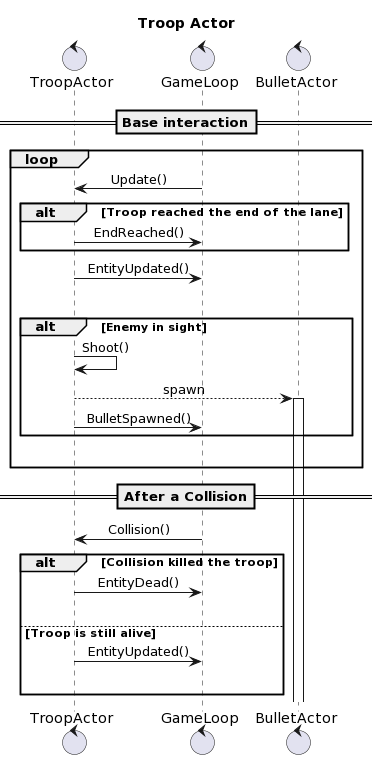
\includegraphics[width=\linewidth]{images/troop-actor.png}
    \label{Diagramma di sequenza del Troop Actor.}
\end{figure}

\subsubsection{Plant}


\subsubsection{Wave}